\documentclass[12pt,a4paper,openany]{book}
\newcommand\tab[1][1cm]{\hspace*{#1}}
\usepackage{amsmath,amsthm,amssymb,graphicx,hyperref}
\usepackage[left=1.2in,right=1.2in,top=1in,bottom=1in]{geometry}
%\usepackage[romanian]{babel}
\usepackage[english]{babel}
\usepackage[table]{xcolor}
\usepackage{tabularx}
\usepackage{multirow}
\usepackage{caption}
\definecolor{captiongray}{gray}{0.35}
\DeclareCaptionFont{captiongray}{\color{captiongray}}
\captionsetup{
    font={small,captiongray},
    labelfont={bf,captiongray},
    justification=centering,
    singlelinecheck=true
}
\usepackage{paralist}
\RequirePackage{hyphenat}
\usepackage{algorithmic, algorithm}
\usepackage[inline]{enumitem}
\usepackage{float}
%\usepackage{...insert other packages here...}
\newtheorem{thm}{Theorem}[section]
\newtheorem{lem}[thm]{Lemma}
\theoremstyle{definition}
\newtheorem{defn}{Definition}[section]
\theoremstyle{remark}
\newtheorem{rem}{Remark}[section]
\newtheorem{exmp}{Example}[section]
\begin{document}
\sloppy

\thispagestyle{empty}
\begin{center}
\begin{figure}[h!]
\vspace{-20pt}
\begin{center}

\includegraphics[width=100pt]{En/INFO_Asset-1.png}
\end{center}
\end{figure}


{\large{\bf WEST UNIVERSITY OF TIMI\c SOARA

FACULTY OF COMPUTER SCIENCE

INTELLIGENT SOFTWARE ROBOTICS}}

\vspace{120pt}
{\huge {\bf MASTER THESIS}}

\vspace{160pt}
\end{center}

{\large\noindent{\bf SUPERVISOR:
\hspace{172pt} GRADUATE: }

\noindent Lect. Dr. Alin Brîndușescu \hfill 
\noindent  Aurel-Ionuț Coruian
}

\vfill
\begin{center}
{\bf TIMI\c SOARA

2026}
\end{center}
\newpage
\thispagestyle{empty}
\begin{center}
{\large{\bf WEST UNIVERSITY OF TIMI\c SOARA
		
FACULTY OF COMPUTER SCIENCE
		
INTELLIGENT SOFTWARE ROBOTICS}}

\vspace{200pt}
{\huge {\bf Implementation of a Real-Time Multi-User Neurofeedback System for Classroom Engagement Monitoring }}

\vspace{153pt}
\end{center}

{\large\noindent{\bf SUPERVISOR:\hfill GRADUATE:}

\noindent Lect. Dr. Alin Brîndușescu \hfill 
\noindent  Aurel-Ionuț Coruian
}

\vfill
\begin{center}
{\bf TIMI\c SOARA

2026}
\end{center}

\newpage
\normalsize{}

\section*{Abstract}


This thesis explores the possibility of developing a multi-user neurofeedback system designed for classrooms, using low-cost, single-electrode Brain-Computer Interface devices (BCI). We opted to use the NeuroSky MindWave Mobile 2 headsets for this study. The system will aim to collect and process attention data from multiple students in real time, giving educators an insightful overview of student focus and engagement throughout different segments of a lecture.


The architecture of the system is built around a network of BCI headsets transmitting data through a Lab Streaming Layer (LSL) protocol, to a computer that will be operated by the teacher in the front, something that most personnel already have at hand. A dedicated Python application will also be implemented, with the goal of visualizing each student’s attention level dynamically, enabling the instructor to identify not only patterns of engagement, but also of disengagement. The system also allows lectures to be segmented into predefined sections, correlating attention levels with specific parts of the material. This system helps with post-lecture analysis to determine which topics or segments sustained the most (or least) student interest, supporting educators to do data-driven adjustments in their teaching strategies.


Contrary to most papers on this theme, the focus of this thesis is not on analyzing learning outcomes or comparing teaching methodologies, but rather on evaluating the technical and practical feasibility of such a system in a classroom context and how it can influence learning as a whole. This work investigates aspects such as data synchronization, signal quality, scalability, and user experience, giving us a foundation for future research in neurofeedback-based education utilizing this system. Ultimately, this project aims to contribute toward the development of intelligent educational tools that leverage neurotechnology to improve teaching effectiveness and engagement of students.
\let\cleardoublepage\clearpage

\newpage
\section*{Statement of Scientific Integrity}

I declare that this MSc thesis is an original report and represents my own work, conducted under the supervision of Lect. Dr. Alin Brîndușescu. All research methods, data collection, analysis and interpretation presented in this thesis are accurately reported and all sources have been cited appropriately where I have made use of ideas and/or visuals of others.

I used generative AI during the writing and research process. The details are presented in the Generative AI Tools Usage section.

\let\cleardoublepage\clearpage

\tableofcontents
\let\cleardoublepage\clearpage

\chapter{Introduction}\label{cap:intro}
Brain–Computer Interface (BCI) technologies have been developing really fast, and they now let us see what’s going on in the brain almost in real time. In classrooms, this could give us a better idea of how students pay attention, stay engaged, or handle mentally difficult tasks. Using neurofeedback, teachers could actually measure attention, notice when students get tired, and maybe even adjust their teaching on the spot to help everyone follow along better. In this thesis, I look at how a multi-user neurofeedback system could work in practice, collecting attention data from students during lessons and giving a way to make teaching a bit more personalized and based on real data, not just guesses.



\section{Motivation}\label{sect:mot}
Modern education has achieved significant advances, incorporating new teaching tools and pedagogical strategies. However, a persistent challenge remains: the limited individualization of instruction. Most classrooms still follow a “one-method-fits-all” approach, and research on student engagement often relies on group-level analysis rather than individual metrics. Neurofeedback offers a promising solution to this limitation, as it allows for continuous, individualized monitoring of attention and cognitive load during learning activities. By capturing real-time neural data, teachers and researchers can gain a better understanding of how each student interacts with course material and identify segments of instruction that are more or less engaging \cite{Apicella2022}.


This approach not only supports individualized feedback but also informs the design of adaptive learning environments that maintain overall class cohesion. For example, electroencephalogram (EEG) based attention monitoring can reveal some patterns of disengagement that might usually go unnoticed, making it possible to have timely interventions such as content adjustment or brief focus exercises. Furthermore, neurofeedback provides value for students with special needs, such as those with dyslexia or other attention-related difficulties, giving educators a way to tailor tasks that are challenging to become more manageable for them.


By integrating neurofeedback into classroom settings, this work aims to bridge the
gap between broad educational strategies and individual cognitive profiles. The
result is a data-informed foundation that supports more effective and responsive
teaching while preserving a collective learning environment \cite{Marzbani2016}.

\section{Research Objectives}\label{sect:robj}
The main objective of this thesis is to explore whether a multi-user neurofeedback system can function reliably in a real classroom setting, using low-cost, single-electrode BCI headsets. The device range the project actually targets is this affordable, single-electrode kind, such as the NeuroSky MindWave, since the whole point is to keep a classroom deployment cheap. For this prototype, however, an 8-channel Unicorn headset was used, simply because that was the equipment already available at the university. The Unicorn is a more expensive, research-grade device, but for the purpose of this work the two are interchangeable: only a single channel and a single attention metric are needed, so the same setup would run just as well on the cheaper single-electrode hardware it is ultimately meant for. Since educational environments are unpredictable—students move, talk, shift attention, and produce a lot of noise—the first goal is simply to determine if attention signals can be captured, synchronized, and visualized in real time without requiring complex equipment or laboratory-grade conditions. This involves evaluating the stability of data transmission through the Lab Streaming Layer (LSL) protocol, the consistency of the attention metric provided by the headsets, and how well multiple devices can operate simultaneously on the same network.


A second objective is to design and implement a software pipeline that enables teachers to observe attention patterns while a lesson is happening. The thesis aims to build an interface that updates dynamically and displays each student’s attention level in a way that is easy to interpret without requiring technical expertise. Another part of this objective is to allow lessons to be divided into labeled segments, so that the collected attention data can later be linked to specific topics or activities from the class. This makes the system useful not only in real time but also as a tool for reflecting on which parts of a lecture were more engaging or more difficult.


Finally, this work aims to understand how such a system could fit practically into everyday teaching. The objective is not to decide whether neurofeedback improves learning or not, but to see how feasible it would be for teachers to use such technology without interrupting their way of working. This includes evaluating aspects like setup time, headset comfort, data clarity, and how easily they can interpret the visualizations.

\section{Brain–Computer Interfaces Overview}\label{sect:bciov}
BCI signal-processing pipelines generally follow a sequence of acquisition, preprocessing, feature extraction, and interpretation. This structure is well established in foundational BCI research, where data quality at the acquisition stage is strongly influenced by electrode placement, impedance control, amplifier characteristics, and sampling rate constraints \cite{Wolpaw2012}. In practical environments such as classrooms, hardware limitations—especially reduced channel counts and portability-focused designs—directly affect the spectral information available for later analysis.


Preprocessing aims to reduce noise sources such as muscle contractions, eye movements, and environmental interference. Typical operations include band-pass filtering, notch filtering, and spatial transformations like the Common Average Reference. The effectiveness of these techniques becomes particularly important in non-laboratory settings, where movement and variability among users introduce additional noise.


Feature extraction commonly relies on frequency-domain representations of neural activity. Well-documented relationships exist between oscillatory patterns and cognitive states: alpha rhythms are associated with fluctuating attentional demand, theta activity is linked to memory and task difficulty, and beta rhythms often reflect executive processes or sustained engagement \cite{Niedermeyer2005}.


In multi-user setups, additional challenges arise, including the need for consistent timing across devices and maintaining stable data quality despite variations in headset placement and user behavior. While the underlying principles remain the same, scaling a system to multiple participants increases sensitivity to synchronization issues, hardware drift, and differences in electrode contact.

\section{Educational Relevance}\label{sect:edurel}
Understanding cognitive engagement in classrooms is a long-standing challenge in educational research. Traditional methods, such as observations or self-report questionnaires, provide only indirect or retrospective measures of student attention, which are often influenced by subjectivity and social desirability \cite{DMello2013}. Neurofeedback and EEG-based monitoring offer a complementary approach by capturing continuous, objective indicators of mental states in real time, enabling instructors to identify when students are attentive, fatigued, or cognitively overloaded.


In addition to physiological approaches, intelligent tutoring systems have
explored alternative methods for assessing student engagement and learning
processes. Systems such as AutoTutor incorporate natural language interaction
and user modeling to estimate both cognitive and affective states during learning
activities. These approaches highlight the importance of continuously monitoring
student responses and adapting instructional strategies accordingly, rather than
relying solely on static or retrospective evaluation methods \cite{DMello2013}.


Previous research has shown that neural activity correlates with attention and cognitive processing dynamics, supporting its use as an objective indicator of engagement. \cite{Dmochowski2014}.


These approaches collectively highlight the growing importance of integrating objective, real-time measurements of cognitive states into educational environments, motivating the development of systems that can provide actionable insights for both instructors and learners.
\chapter{Related Work}\label{cap:relwork}
Before presenting the proposed system, the thesis must be placed in the context of existing work on EEG-based monitoring and neurofeedback in education. The studies reviewed in this chapter show both the potential of portable EEG devices and the practical difficulties that appear when such systems are moved outside controlled laboratory conditions. Particular attention is given to multi-user acquisition, cognitive engagement metrics, and simplified attention measures, because these aspects directly influence the design choices made later in the project.



\section{Literature Review}\label{sect:litrev}
Recent studies have shown that EEG monitoring can support educational research by offering objective measures related to attention and cognitive load. Portable and more affordable EEG devices have been applied in studies involving reading, arithmetic tasks, and relaxation exercises \cite{Emri2023}. These results suggest that EEG activity, especially in the alpha, beta, and theta bands, can reflect changes in attention and cognitive effort, making it useful for studying learning dynamics in more practical environments.


Multi-user EEG systems have also been proposed for capturing synchronized attention data from several students at the same time \cite{Apicella2022}. By combining wireless headsets with real-time data streaming, these systems make it possible to visualize class-level engagement and identify trends across different segments of instruction. At the same time, they show why signal processing, artifact handling, and synchronization are important when EEG measurements are used in educational settings \cite{Marzbani2016}.


Other research has examined whether EEG data can be collected from multiple participants in realistic classroom environments. Poulsen et al. demonstrated that synchronized neural recordings can be obtained from groups of students using portable EEG devices during shared learning activities \cite{Poulsen2017}. Their work highlights the challenges caused by differences between users and by environmental noise, but it also supports the feasibility of classroom-scale EEG monitoring.


Simplified EEG setups form another relevant research direction. Studies based on single-channel EEG have shown that attention-related features can still be extracted even when the hardware configuration is minimal \cite{Liang2022}. Although such systems provide less spatial information and are more sensitive to artifacts, they offer advantages in cost, usability, and scalability. These qualities make them relevant for educational environments, where complex laboratory setups are rarely practical.


Broader analyses of portable EEG technologies in education emphasize both the opportunities and the limitations of these systems. Reviews in this area point out that portable devices enable more flexible and accessible experimentation, but issues such as signal quality, lack of standardization, and interpretation of cognitive metrics remain open challenges \cite{Xu2018}.


Taken together, these works provide the foundation for the system presented in this thesis. They support the use of portable EEG in educational contexts, while also showing why a classroom prototype must prioritize practical deployment, readable visualization, and careful interpretation of engagement indicators.

\section{Cognitive Engagement Metrics}\label{sect:cognmet}
Cognitive engagement is not a directly observable variable, which makes its measurement difficult in educational systems. In the literature, it is usually inferred from signals that are associated with attention, mental effort, task involvement, or sustained processing. EEG is useful in this context because it captures neural activity continuously and with high temporal resolution, allowing changes in engagement to be followed during a task rather than only after it has ended \cite{Wolpaw2012}.


Many EEG-based engagement metrics rely on spectral information. Classical EEG research describes several frequency bands that are relevant for cognitive interpretation, including theta, alpha, and beta activity \cite{Niedermeyer2005}. These bands are not simple labels for attention, but they provide a useful starting point. In general terms, theta activity is often discussed in relation to cognitive control and task demand, alpha activity is frequently associated with relaxation or reduced cortical activation, and beta activity is often linked with active processing and alertness. Because these relationships depend on context, band power should be interpreted carefully rather than as a direct measurement of learning.


A well-known engagement formulation is the beta-to-alpha-theta ratio. Pope et al. evaluated several EEG indices in a biocybernetic system and found that the ratio between beta power and the sum of alpha and theta power was the most suitable candidate among the tested engagement indices \cite{Pope1995}. Later work also connected EEG-derived engagement and workload measures with task performance, vigilance, memory, and mental effort, showing that such indicators can follow changes in cognitive state over time \cite{Berka2007}.


For classroom applications, however, the usefulness of a metric depends not only on its theoretical relevance, but also on its practical stability. Liang et al. compared attention-related features in single-channel EEG systems and showed that simplified setups can still provide useful information for attention monitoring \cite{Liang2022}. This is important for educational prototypes, because classroom systems must balance signal quality with comfort, cost, and ease of deployment.


The metric used in this thesis follows this practical direction. It uses a simple spectral ratio because the goal is to provide a transparent engagement indicator, not to build a clinical diagnostic model. This choice is consistent with the related work: EEG engagement indices can be informative, but they should be treated as approximate indicators that require context and human interpretation.

\section{Neurofeedback in Education}\label{sect:neurfbedu}
Neurofeedback systems use physiological measurements to provide feedback about cognitive or affective states. In a strict clinical sense, neurofeedback often involves training users to regulate their own brain activity. In educational technology, the term is sometimes used more broadly, referring to systems that monitor neural or physiological signals and use them to support learning, adaptation, or reflection.


Marzbani et al. describe neurofeedback systems as pipelines that include signal acquisition, preprocessing, feature extraction, feedback generation, and evaluation \cite{Marzbani2016}. This general structure is relevant for classroom prototypes as well, even when the feedback is directed mainly to the teacher rather than directly to the student. The same basic problem remains: noisy physiological data must be transformed into information that can be understood and used in a meaningful way.


In educational settings, EEG-based feedback has been explored as a way to make engagement less dependent on self-report or manual observation. Apicella et al. developed an EEG-based measurement system for monitoring student engagement in Learning 4.0, showing how wearable acquisition and real-time visualization can be combined to support classroom awareness \cite{Apicella2022}. Their work is especially relevant because it treats engagement monitoring as part of a teaching environment rather than as an isolated laboratory task.


Neurofeedback also connects to a wider research direction in adaptive learning systems. Intelligent tutoring systems such as AutoTutor use information about cognitive and affective states to adapt interaction and support learning \cite{DMello2013}. Although these systems do not necessarily rely on EEG, they illustrate the broader educational motivation: learning environments become more useful when they can respond to the learner's current state instead of applying the same strategy throughout the whole session.


Recent reviews of wearables for engagement detection show that physiological monitoring in learning environments is not limited to EEG. Heart rate, skin temperature, electrodermal activity, eye tracking, posture, and other signals have also been used to estimate engagement or emotion \cite{BustosLopez2022}. This broader context is useful because it shows that EEG should not be treated as the only possible source of engagement information. For this thesis, EEG was selected because it is directly related to neural activity and can be streamed in real time, but a future system could combine it with additional signals.

\section{Limitations of Current Approaches}\label{sect:limcurrapp}
Despite the promise of EEG-based engagement monitoring, several limitations appear consistently in the literature. The first is signal quality. Portable EEG devices are easier to use than laboratory equipment, but they normally have fewer channels, weaker spatial information, and greater sensitivity to movement and electrode contact problems \cite{Xu2018}. These limitations become more visible in classrooms, where students naturally move, talk, and interact with their environment.


Multi-user acquisition introduces additional difficulties. Poulsen et al. showed that synchronized EEG recordings can be collected from groups of students during classroom-like activities, but their work also highlights variability between participants and the need for robust processing \cite{Poulsen2017}. In practice, a classroom system must handle imperfect headset placement, different levels of movement, and streams that may start or stop at different times.


Another limitation concerns interpretation. Engagement is a complex construct with cognitive, behavioral, and affective components. A single EEG value cannot fully represent whether a student understands the lesson, is motivated, is confused, or is simply physically still. Reviews of wearable engagement detection emphasize this diversity of signals and meanings, showing that engagement monitoring is useful but not straightforward \cite{BustosLopez2022}.


There is also a methodological risk in over-automating interpretation. If EEG-derived values are presented as exact measures, teachers may be encouraged to rank students or draw conclusions that the signal cannot support. For this reason, related work supports a cautious approach: engagement indicators can provide additional information, but they should be combined with pedagogical judgement, lesson context, and awareness of signal limitations \cite{Xu2018,Liang2022}.


These limitations directly influence the system proposed in this thesis. The prototype does not attempt to diagnose attention or evaluate students automatically. Instead, it presents engagement as a contextual indicator, keeps technical inspection available, and supports post-lesson reflection. This makes the system more realistic for a master's-level prototype and more appropriate for educational use.

\section{Attention Measurement Techniques}\label{sect:attmeasteq}
Attention can be measured through several techniques, each with different strengths and weaknesses. Traditional educational methods include observation, questionnaires, and performance analysis. These methods are easy to apply, but they are often retrospective or subjective. Physiological methods, including EEG, add continuous measurement, but they require careful acquisition and interpretation.


Within EEG-based approaches, one common technique is band-power analysis. The signal is divided into frequency bands, and changes in power are used as features for estimating cognitive state \cite{Niedermeyer2005}. This method is relatively simple and computationally efficient, which makes it suitable for real-time prototypes. The engagement ratio used by Pope et al. is an example of this type of technique, because it combines beta, alpha, and theta power into a single index \cite{Pope1995}.


Another technique is feature comparison or fusion. Liang et al. evaluated attention-related features in single-channel EEG systems and proposed feature fusion to improve attention monitoring \cite{Liang2022}. This direction is useful when the system has limited hardware but still needs a more reliable estimate than a single raw feature can provide. Such methods can improve performance, but they also add complexity and may require more validation data than is available in a small prototype.


Multi-user classroom research has also used inter-subject correlation. Dmochowski et al. showed that temporal reliability of neural responses to naturalistic stimuli can predict audience preferences, and Poulsen et al. later applied related ideas to synchronized EEG recordings in a classroom setting \cite{Dmochowski2014,Poulsen2017}. This technique is powerful for group-level analysis, especially when students are exposed to the same stimulus, but it is less direct for displaying an individual live engagement value for each student.


The attention measurement technique adopted in this thesis is therefore deliberately simple. It uses spectral information to compute an engagement indicator that can be updated in real time and explained clearly. This does not make it the most advanced possible technique, but it matches the goals of the prototype: real-time operation, multi-user support, readable visualization, and cautious interpretation.

\chapter{System Design}\label{cap:sysdes}
Following the requirements and constraints established in the previous chapters, the proposed solution was designed as a modular classroom prototype. Its purpose is not to function as a fully automated assessment platform, but to connect student-side EEG acquisition, local stream transport, teacher-side processing, and post-lesson review into a coherent workflow for observing engagement during teaching activities.



\section{Concept Overview}\label{sect:concov}
At concept level, the system gives the teacher an additional source of information about classroom engagement during technology-supported lessons. It does not replace teacher judgement, evaluate students automatically, or make definitive claims about learning outcomes. Instead, it collects EEG samples from participating students, converts them into an engagement indicator, and presents the result in a form that supports reflection on lesson pacing, topic difficulty, and moments where attention may decrease. The value is treated as an indicator rather than an absolute measurement, since classroom EEG is influenced by movement, electrode contact, individual variation, and environmental noise; this cautious interpretation follows previous classroom EEG studies, where engagement monitoring is treated as supportive information rather than as a direct measure of learning \cite{Poulsen2017,Apicella2022,Xu2018,BustosLopez2022}.


In the intended classroom scenario, each student uses one Unicorn EEG headset connected to one Raspberry Pi acquisition node, and this station is repeated for \(N\) students, with every station publishing its stream to the same local network. The student-side node is kept deliberately simple: its role is limited to acquisition and transmission, without any pedagogical decision-making. On the teacher workstation, the application receives the available streams, identifies them by student or device label, computes the engagement value, and displays the information through a Streamlit interface. Keeping interpretation, visualization, lesson management, and reporting on the workstation creates a complete path from physiological acquisition to classroom-facing feedback, and means that changes to the metric or to the interface do not require the acquisition nodes to be redesigned.


The interface is teacher-centered: rather than ranking students or building permanent profiles, it focuses on lesson activity and class-level reflection, so the teacher can relate changes in engagement to instructional decisions without reducing students to a single numerical score. Because a live signal monitor alone would not be sufficient for this, the prototype also includes the surrounding teaching workflow, where materials can be uploaded, previewed, presented, and later reviewed through reports. EEG-derived engagement becomes more meaningful this way: a decrease during a particular slide is more useful when the teacher can relate it to the topic or activity taking place at that moment.

\section{Architecture and Data Flow}\label{sect:archndf}
Architecturally, the prototype is organized around four main parts: acquisition nodes, stream transport, teacher-side processing, and local storage. Acquisition nodes interact with the EEG headsets, the transport layer makes streams discoverable on the local network, the teacher application receives and interprets the data, and local storage preserves lesson materials, generated previews, configuration data, and report information. This separation gives the system a clear structure and allows each part to be tested with limited dependence on the others.


Data flow begins at the student-side unit. The Unicorn headset provides the EEG signal, and the paired Raspberry Pi acquisition node forwards that signal as an LSL stream. Stream metadata identifies the device and student label, which allows the teacher application to distinguish between several participants. By using distributed acquisition nodes, the teacher workstation does not need to manage direct headset connections, which would become increasingly difficult as more students are added.


When a stream becomes available on the local network, the teacher application discovers it and opens a receiving inlet. Incoming samples are stored in a stream state containing the current signal value, packet count, connection freshness, stream metadata, and in-session history. The attention-processing component receives the selected EEG values and produces an engagement estimate, while the user interface reads the organized state and presents it through cards, detail views, charts, and reports.


This stream state functions as the main internal representation on the teacher side. Interface pages do not work directly with network connections; they work with structured information about each detected participant stream. Such an arrangement makes the visual layer more stable, because streams can appear, become quiet, or disappear without forcing the whole interface to change its structure.


Classroom conditions also motivated a tolerant startup model. A lesson can be prepared even when no headset is currently streaming. A Raspberry Pi can be deployed or validated from the administration page before teaching begins. New streams may also appear after the teacher application has already started, because discovery is performed dynamically. This flexibility is useful in practical teaching environments, where setup time is limited and devices may not all become available at the same moment.


Two information paths meet inside the teacher application. One path is physiological: headset, acquisition node, LSL stream, collector, attention metric, visualization. The other is instructional: uploaded material, local preview, presentation, report. Bringing these paths together prevents engagement information from being shown in isolation and makes it possible to relate the signal to the activity taking place during the lesson.

Figure~\ref{fig:hardware_deployment} presents the hardware side of this separation. The left part of the diagram represents one student station: the student wears the Unicorn headset, the Raspberry Pi reads the device through the vendor library, and the Pi streamer publishes the resulting signal. This station is repeated for each participant, while the teacher workstation remains the single point where the streams are observed and interpreted.

\begin{figure}[h]
\centering
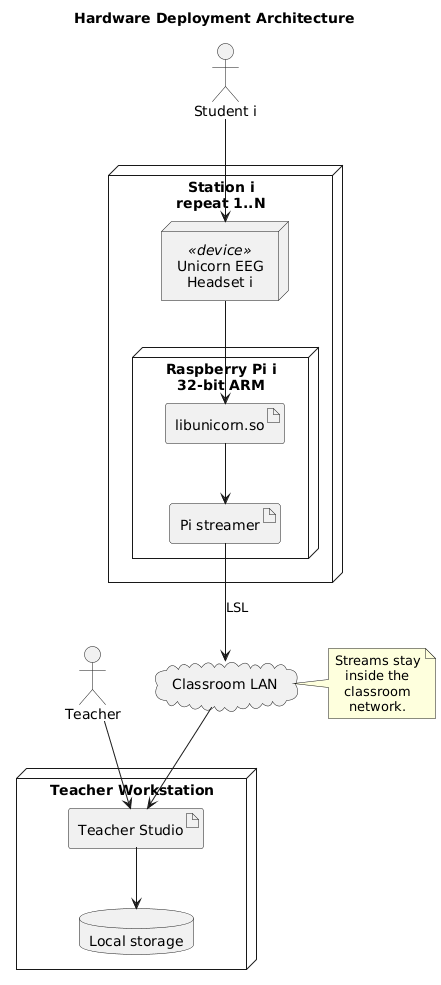
\includegraphics[width=0.82\textwidth,height=0.68\textheight,keepaspectratio]{En/UML_hardware_diagram.png}
\caption{Hardware deployment architecture for the classroom prototype. Each student station contains one Unicorn headset and one Raspberry Pi acquisition node, while the teacher workstation receives the resulting LSL streams over the classroom network.}
\label{fig:hardware_deployment}
\end{figure}

The classroom workflow is intentionally sequential from the teacher's perspective: setup and validation happen before the lesson, while monitoring, presentation, and report review happen during and after teaching. Figure~\ref{fig:application_flow} summarizes this operational flow.


\begin{figure}[h]
\centering
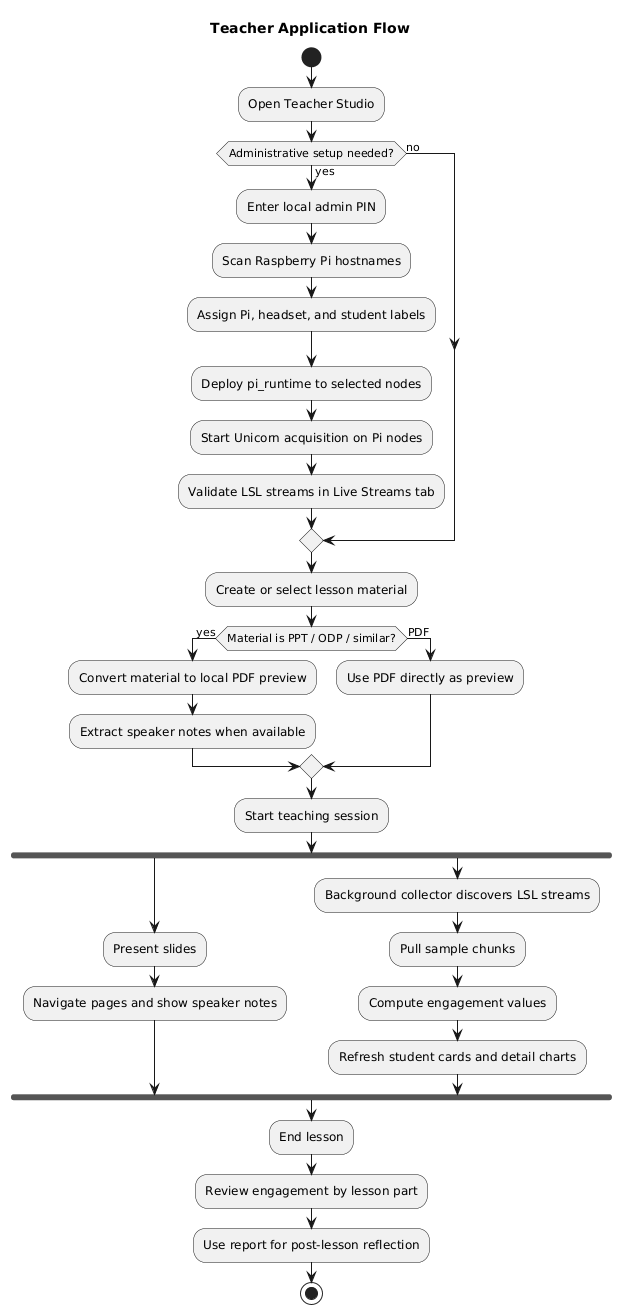
\includegraphics[width=0.82\textwidth,height=0.68\textheight,keepaspectratio]{En/UML_app_flow.png}
\caption{Application workflow from device preparation and stream validation to lesson presentation and post-lesson review.}
\label{fig:application_flow}
\end{figure}

The activity diagram is useful because it shows that the prototype is not only a signal viewer. It starts with administration tasks such as device preparation and stream validation, then moves into lesson selection and presentation, and only after the lesson does it enter the reporting stage. This matches the way the application is intended to be used in a real teaching session.


\section{Hardware Setup}\label{sect:hwset}
For the hardware layer, the prototype uses a distributed acquisition model. Instead of connecting all EEG devices directly to the teacher workstation, each student-side headset is paired with a nearby Raspberry Pi node, forming one acquisition station for that student. You can see an example of such a station in Figure~\ref{fig:hardware_setup} A classroom deployment can contain \(N\) such stations, but a single student does not share or control multiple stations. The Pi handles device access and stream publication, while the teacher workstation receives standardized streams over the local network. In a classroom setting, this reduces the amount of direct hardware management required on the teacher computer.

As signal source, the system uses the Unicorn EEG headset. The Raspberry Pi acts as a compact acquisition computer that runs the device interface and publishes the resulting stream. Each acquisition point can therefore be treated as an independent unit. If another participant is added, another acquisition node can be prepared without changing the teacher-side architecture.

\begin{figure}[h]
\centering
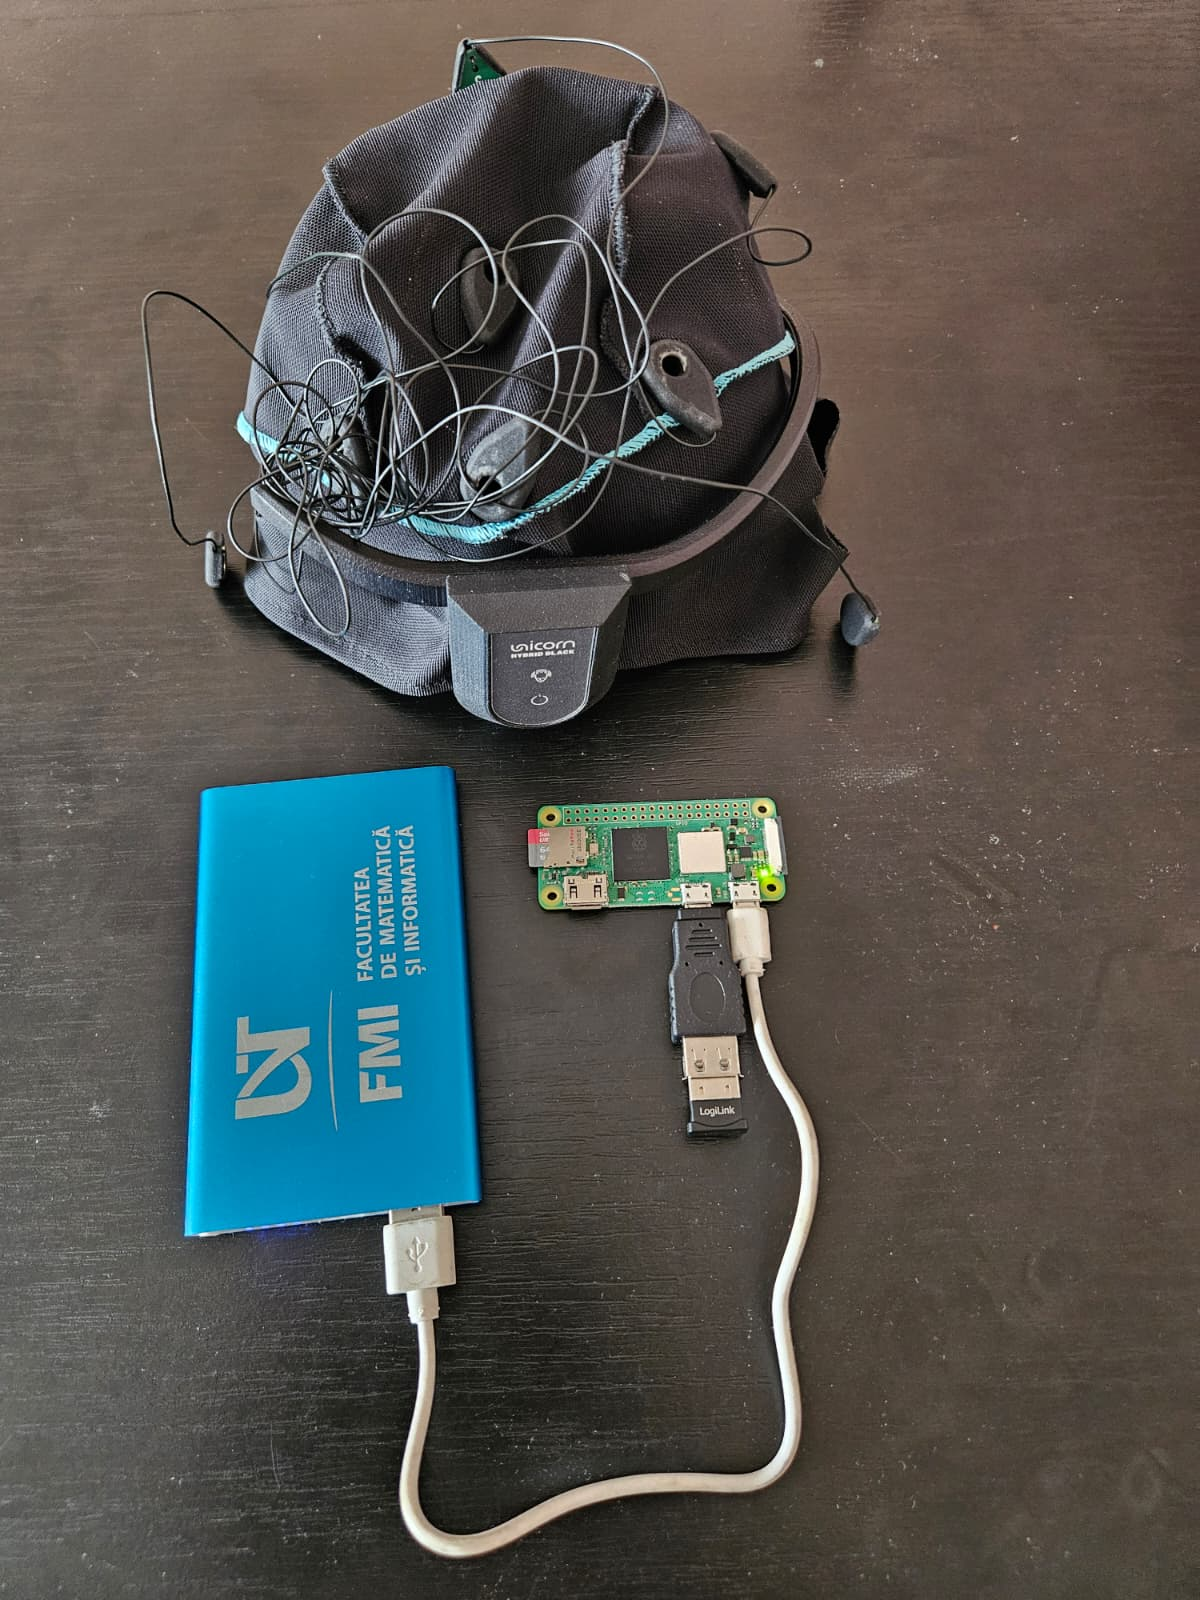
\includegraphics[width=0.92\textwidth]{En/1. Student Station.jpeg}
\caption{Student acquisition station setup showing only the power bank, Raspberry Pi, and Unicorn EEG headset.}
\label{fig:hardware_setup}
\end{figure}

This organization also gives more freedom in classroom placement. The acquisition node can remain close to the student-side device, while the teacher workstation can stay where the lesson is controlled. A design based on direct connections between all headsets and one central machine would be less convenient and more fragile in a normal classroom arrangement.


A practical constraint comes from the vendor library used by the acquisition runtime. The included Unicorn Pi Zero W library targets a 32-bit ARM environment, so the Raspberry Pi setup must be compatible with that requirement. Before any network streaming or signal handling can take place, the acquisition node must be able to load the native library and communicate with the headset.


On the teacher side, the workstation is a standard Windows computer running the Python environment and the Streamlit application. It receives LSL streams, manages lesson materials, runs the engagement processing, and displays the interface. Since no EEG device has to be connected directly to this computer, the setup remains closer to a normal classroom laptop than to a laboratory acquisition station.


Real-time communication is intended to remain local. The core classroom workflow does not depend on cloud services, which makes the prototype usable even when internet access is limited or unreliable. Internet connectivity may still be needed for installation or dependency setup, but teaching, streaming, processing, and review are designed to operate within the local environment.

\section{Software Components}\label{sect:swcomp}
From a software perspective, the system is divided into an acquisition runtime and a teacher application. The runtime executes on the Raspberry Pi and exposes headset data through LSL. The teacher application runs on the workstation and contains the collector, processing module, user interface, lesson services, report view, and administration tools. This division keeps the embedded side focused while placing the more complex interaction logic on the machine used by the teacher.


Figure~\ref{fig:software_architecture} gives the general software organization. The Raspberry Pi side is limited to the bridge between the Unicorn device and the LSL outlet. The LSL layer carries both samples and metadata. On the workstation, the teacher application is split into pages, live acquisition logic, lesson/report services, administration services, and reusable UI components.

\begin{figure}[h]
\centering
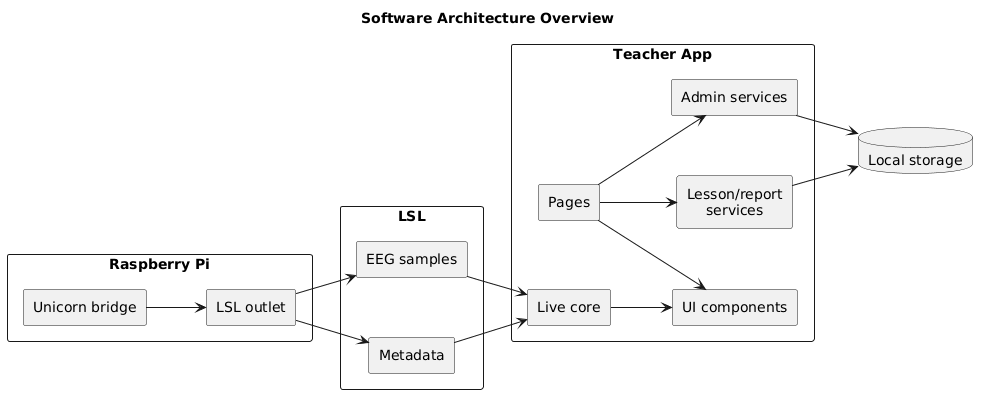
\includegraphics[width=0.92\textwidth]{En/UML_software_diagram.png}
\caption{General software architecture showing the Raspberry Pi runtime, LSL transport, teacher application modules, and local storage.}
\label{fig:software_architecture}
\end{figure}
Within the acquisition runtime, the main responsibility is bridging the native device library and the LSL network. It opens the headset, selects the configured stream mode, attaches metadata, and publishes the signal. The component does not need to know how lessons are presented or how reports are generated, which keeps it reusable and easier to debug.


The acquisition runtime is shown in more detail in Figure~\ref{fig:software_pi_runtime}. The launcher starts the C API streamer, the streamer accesses the vendor library through Python bindings, and the outlet publishes the signal to the classroom network. Keeping this chain short makes failures easier to isolate: device access problems remain on the Pi side, while visualization and interpretation remain on the teacher workstation.

\begin{figure}[h]
\centering
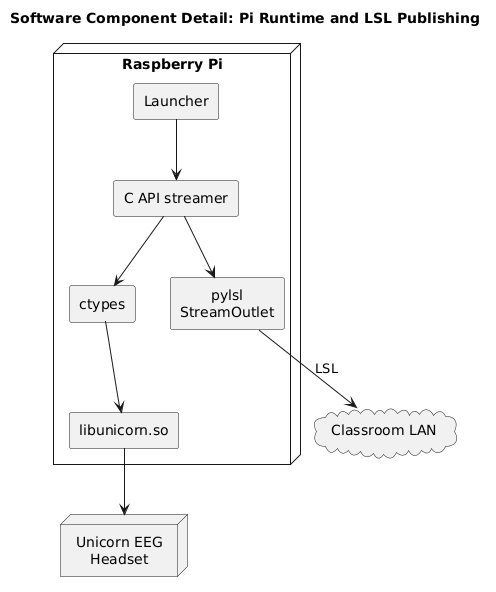
\includegraphics[width=0.7\textwidth]{En/UML_software_pi_runtime.png}
\caption{Pi-side software components used to access the Unicorn device and publish EEG samples through an LSL outlet.}
\label{fig:software_pi_runtime}
\end{figure}

On the workstation, the teacher application is organized into pages and supporting services. Pages define the visible workflow: dashboard, lesson creation, teaching, reports, and administration. Services handle operations such as saving uploaded materials, preparing previews, extracting speaker notes, collecting LSL streams, and deploying acquisition nodes. This prevents the interface from becoming a single block of mixed presentation and system logic.


Signal interpretation is kept independent from the interface. The attention-processing component receives numerical EEG samples and returns an engagement value. Keeping this logic separate makes the metric easier to explain and isolates the signal-processing assumptions from the rest of the application. In future work, a different metric could be introduced without redesigning the lesson pages or the administration workflow.


Figure~\ref{fig:software_live_monitoring} shows the live monitoring path inside the teacher application. The collector service provides access to a background collector, the collector reads LSL samples and metadata, and the attention metric produces engagement updates. The UI does not communicate directly with LSL; it renders snapshots of the stream state, which keeps the interface responsive even when streams appear, become quiet, or disappear.

\begin{figure}[h]
\centering
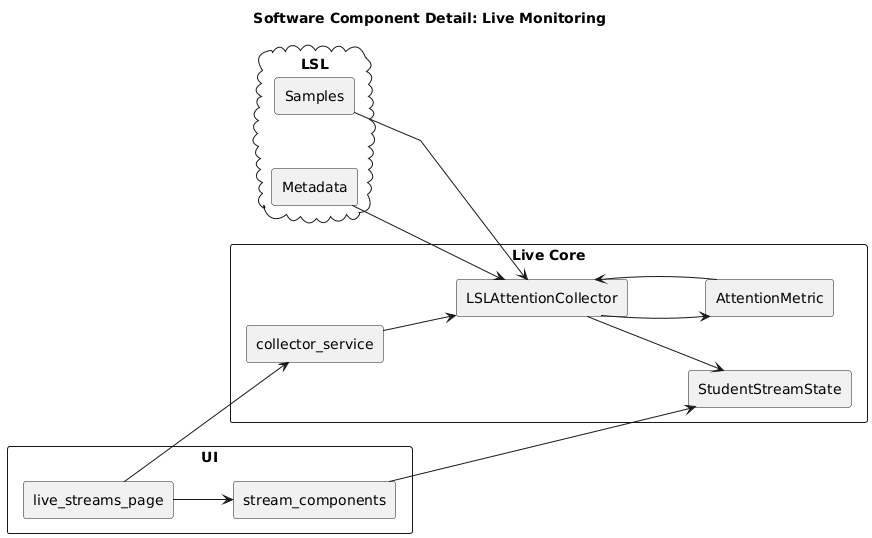
\includegraphics[width=0.9\textwidth]{En/UML_software_live_monitor.png}
\caption{Live monitoring components responsible for receiving LSL streams, maintaining stream state, computing engagement values, and rendering the stream inspection interface.}
\label{fig:software_live_monitoring}
\end{figure}

Lesson and report features complete the teacher workflow. Materials are stored locally and can be presented from inside the same application, while reports summarize engagement by lesson part for later review. Together, these components turn the prototype into a coherent teaching tool rather than a collection of unrelated utilities.


Figure~\ref{fig:software_lesson_reporting} separates the lesson workflow from the live signal workflow. The lesson store manages saved material and metadata, conversion prepares PDF previews when needed, and speaker-note extraction supports presenter view. The reporting component uses lesson segmentation to relate engagement values to meaningful parts of the lesson instead of showing only a raw time series.

\begin{figure}[h]
\centering
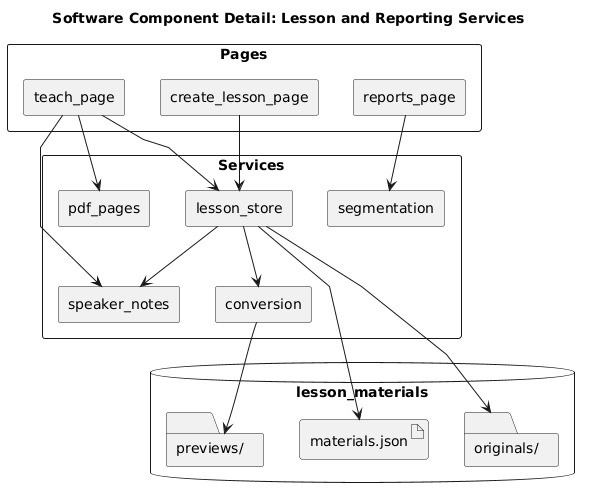
\includegraphics[width=0.88\textwidth]{En/UML_software_lesson_reporting.png}
\caption{Lesson and reporting components used for material upload, preview generation, speaker-note extraction, slide rendering, and post-lesson summaries.}
\label{fig:software_lesson_reporting}
\end{figure}

Administration is included because multi-user acquisition requires preparation before the lesson begins. Devices must be discovered, assigned, deployed, and validated. Keeping these operations in a dedicated area protects the normal teaching pages from unnecessary technical detail while still making setup tasks available when they are needed.

The administration components in Figure~\ref{fig:software_admin_deployment} support this preparation stage. The inventory tab stores Raspberry Pi and headset assignments, the deployment tab uses the PowerShell deployment script to copy and prepare the Pi runtime, and the live streams tab validates that published LSL streams can be discovered by the teacher workstation.

\begin{figure}[h]
\centering
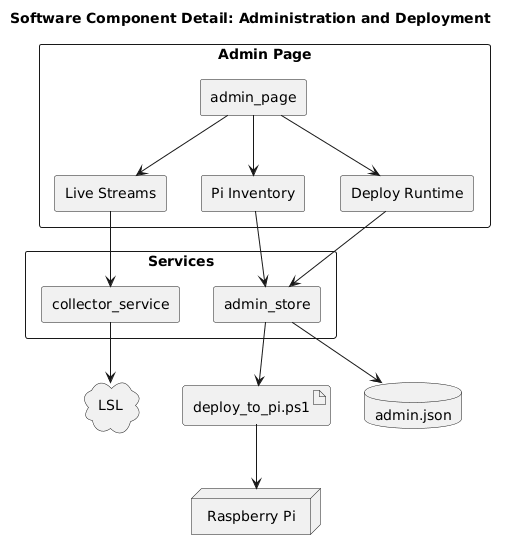
\includegraphics[width=0.8\textwidth]{En/UML_software_admin.png}
\caption{Administration and deployment components used to manage Raspberry Pi inventory, runtime deployment, configuration storage, and stream validation.}
\label{fig:software_admin_deployment}
\end{figure}

\subsection{Lab Streaming Layer Integration}\label{ssect:lsl}
LSL provides the communication boundary between acquisition and interpretation. Each Raspberry Pi publishes a stream, and the teacher workstation discovers and receives available streams on the local network. This avoids custom networking logic and supports a flexible startup order, since acquisition nodes and the teacher interface do not have to be launched in a strict sequence. The choice is also aligned with the intended use of LSL as a framework for timestamped, synchronized data streaming across local networked systems \cite{Kothe2025}.


Metadata attached to the streams is essential for usability. Student labels, device names, channel information, and stream names allow the teacher application to present multiple streams in a readable way. Without this context, the interface would receive numerical samples but would not have enough information to associate them meaningfully with classroom participants.


A further distinction is made between signal timing and interface freshness. LSL timing preserves the meaning of incoming data, while local receipt time helps the interface decide whether a stream appears live, quiet, or stale. In a classroom dashboard, showing whether values are still being updated is almost as important as showing the values themselves.

\subsection{Python Visualization Module}\label{ssect:pyvizmod}
Streamlit was selected for the visualization module because the prototype needs to combine Python-based processing with a usable teacher interface. Its structure follows the teacher's workflow rather than the internal implementation modules. The dashboard gives quick access to the main tasks, while the lesson, teaching, report, and administration pages separate the different moments of use.


The dashboard in Figure~\ref{fig:teacher_dashboard} is the teacher's entry point. It avoids exposing low-level streaming details immediately and instead presents the four main actions: preparing material, teaching, reviewing reports, and entering the administration area. This keeps routine classroom use separate from technical setup tasks.

\begin{figure}[h]
\centering

\includegraphics[width=0.95\textwidth]{\detokenize{En/2. Teacher Dashboard.png}}
\caption{Teacher Studio dashboard with quick access to lesson creation, teaching, reporting, and administration.}
\label{fig:teacher_dashboard}
\end{figure}
Live stream information is shown at two levels of detail. Student cards provide a compact view of engagement and stream status, which is suitable for quick inspection during a lesson. A detailed view exposes raw samples and stream metadata, making it more useful during setup or troubleshooting. This balance is important because normal teaching requires a simple display, while validation sometimes requires deeper technical information.


Figure~\ref{fig:live_stream_cards} illustrates the compact level. Each card combines the student label, engagement value, device identifier, LSL stream name, and freshness status. The stale card is important because it shows how the interface communicates a missing or inactive data source without removing the student from the display.

\begin{figure}[h]
\centering

\includegraphics[width=0.95\textwidth]{\detokenize{En/3a. 4 Student cards with 1 stale.png}}
\caption{Live stream cards showing four configured student streams, including one stale stream where data is no longer being received.}
\label{fig:live_stream_cards}
\end{figure}

\begin{figure}[h]
\centering

\includegraphics[width=0.9\textwidth]{\detokenize{En/3b. Student-01 engagement and metrics.png}}
\caption{Selected-student detail view showing engagement value, stream status, packet count, sample rate, and connection freshness.}
\label{fig:selected_student_metrics}
\end{figure}
Figure~\ref{fig:selected_student_metrics} shows the detailed level for one stream. This view is more technical and is meant for validation or troubleshooting: it exposes packet count, sample rate, last-seen age, status, and the latest engagement value for the selected student.
By connecting lesson activity and engagement monitoring, the interface supports the practical goal of the project. Materials can be prepared, previewed, presented, and later reviewed through reports. Neurofeedback is therefore placed inside the teaching process, rather than being presented as a separate technical instrument that distracts from the lesson.


Unnecessary signal-processing terminology is avoided in the normal teaching flow. Technical details remain available in stream inspection and administration views, but the main workflow is expressed through familiar actions such as creating a lesson, presenting material, and reviewing a report. This makes the system easier to approach in an educational context.

\section{Data Transmission Protocols}\label{sect:commnsync}
Different communication methods are used for live data and management tasks. Real-time EEG samples are transmitted through LSL because they require discovery and timestamped streaming \cite{Kothe2025}. Deployment and maintenance use SSH and SCP, which are more appropriate for remote command execution and file transfer than for continuous signal transmission.


Information that must persist between sessions is stored locally on the teacher workstation. This includes lesson materials, generated previews, configuration files, device inventory, and deployment logs. A local-first design keeps the classroom workflow independent of cloud services and makes the prototype easier to run in a controlled school environment.


Access to administration functions is separated from the normal teaching pages and protected by a local PIN hash. This should not be interpreted as a complete security model for sensitive data, but it provides a basic boundary between everyday teaching actions and technical operations such as deployment or device inventory changes. A production version would require stronger privacy and access-control mechanisms.

\clearpage

\chapter{Implementation and Processing Pipeline}\label{cap:implnprocpipe}
Chapter 4 describes how the proposed architecture was implemented in the working prototype. The discussion follows the data path from headset acquisition to teacher-facing visualization, with emphasis on the practical processing steps that make live engagement feedback possible during a lesson.



\section{Signal Acquisition Process}\label{sect:signacqproc}
Signal acquisition takes place on the Raspberry Pi paired with each headset. In practice, the acquisition runtime acts as a bridge between the Unicorn device and the LSL network. It prepares the required native libraries, opens the EEG device, receives samples through the vendor API, and publishes the resulting stream so that it can be discovered by the teacher workstation. Using LSL for this boundary follows its role in synchronized multimodal recording and local network stream discovery \cite{Kothe2025}.


At startup, the runtime verifies the environment required for LSL streaming and initializes the Unicorn acquisition path. The native library is loaded through Python bindings to the C API, with the required function signatures defined before the device is accessed. Available devices are then discovered, and the selected headset is opened. When no serial number is provided, the first available device is used, which is convenient for simple testing while still allowing explicit selection in a larger setup.


After the device is opened, an LSL outlet is created and descriptive metadata is attached to it. This metadata includes information such as the student label, device name, stream identity, and channel description. Although these fields are not part of the EEG signal itself, they are necessary for a multi-user classroom interface, where several streams must be displayed in a readable and unambiguous way.


During acquisition, samples are read repeatedly from the headset and pushed to the LSL outlet. Engagement is not computed on the Raspberry Pi. Keeping the acquisition loop limited to reading and publishing makes the student-side process shorter and more predictable, while preserving the raw values for the teacher application. If acquisition is interrupted, the runtime attempts to stop the device and release its handle, reducing the risk of leaving the hardware in an inconsistent state for the next session.


Deployment support is part of this pipeline as well. The teacher application can copy the runtime and required vendor files to the Raspberry Pi and prepare the Python environment used by the acquisition node. This is important for a system intended to work with several nodes, because each one must be configured in a consistent way before being used in a lesson.


On the workstation, a background collector completes the acquisition path. It discovers LSL streams, opens receiving inlets, reads available sample chunks, and stores each stream in a structured state. Identification metadata, connection freshness, packet count, latest raw value, latest engagement value, and short-term histories are kept together so that the dashboard can use live data without managing network streams directly.


Responsiveness is especially important because Streamlit reruns page logic frequently. Long-running acquisition work cannot depend on a single page render. By collecting data in the background and exposing snapshots to the interface, the implementation separates continuous signal reception from visual refresh. This makes the live display more reliable and keeps the interface logic easier to follow.

\section{Data Filtering Procedures}\label{sect:datafiltproc}
Filtering is intentionally kept modest in the current prototype. The system does not implement a full laboratory EEG preprocessing chain. Instead, it performs the steps needed for the engagement metric: selecting the relevant channel, buffering samples into analysis windows, removing the constant offset, and estimating spectral content. This reflects the practical compromise often required when portable EEG is used outside controlled laboratory environments \cite{Xu2018}.


Processing begins with basic validation of the incoming sample. Empty values or values that cannot be converted to a numeric form are ignored, which protects the rest of the pipeline from malformed input. This choice keeps the collector robust without adding complex error handling to the real-time path.


Selected values are buffered until enough recent data is available for frequency analysis. Once a processing window is formed, its mean is subtracted. Removing this constant component prevents the engagement estimate from being influenced by a simple voltage offset rather than by variation in the signal.


Frequency-domain analysis is then performed using an FFT. Rather than reconstructing separate filtered signals for each band, the implementation estimates the power contained in the theta, alpha, and beta ranges directly from the transformed window. This approach is compact and suitable for the prototype, because the final metric depends on relative spectral power rather than on the detailed time-domain shape of each band.


Figure~\ref{fig:eeg_processing_pipeline} summarizes the processing path. Incoming samples are first checked and buffered. Once a complete window is available, the mean is removed, spectral power is estimated in the relevant EEG bands, and the beta-to-alpha-theta ratio is converted into the displayed engagement value through scaling, smoothing, and calibration.

\begin{figure}[h]
\centering
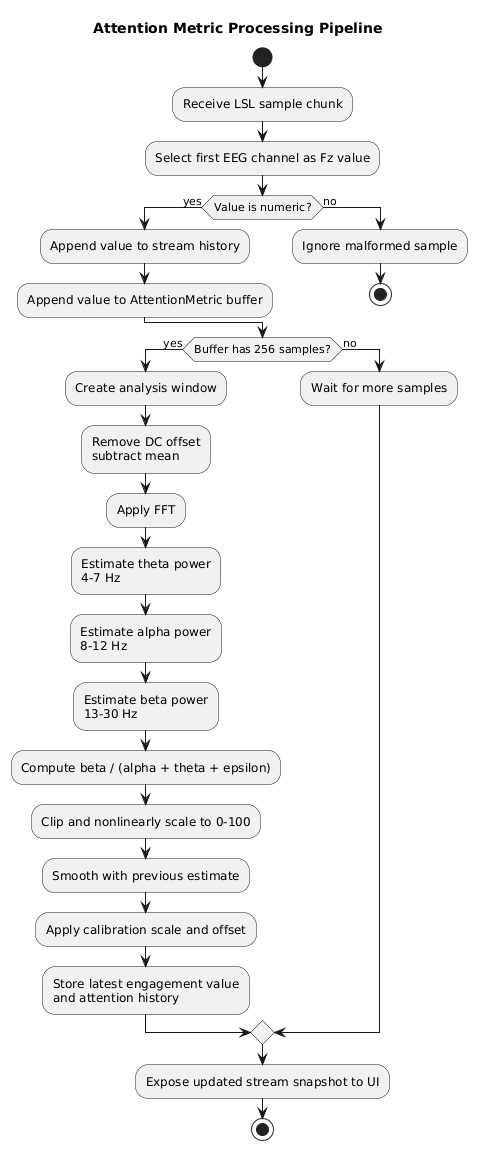
\includegraphics[width=0.82\textwidth,height=0.68\textheight,keepaspectratio]{En/UML_eeg_pipeline.png}
\caption{Processing pipeline used to transform incoming LSL samples into the displayed engagement value.}
\label{fig:eeg_processing_pipeline}
\end{figure}
Not all EEG artifacts are removed by this procedure. Eye movements, muscle activity, poor electrode contact, and normal classroom movement may still influence the signal. This limitation is accepted because the system is a feasibility prototype for real-time classroom feedback, not a clinical acquisition platform. To keep the process transparent, raw sample history is still preserved in the interface, allowing the underlying signal to be inspected when needed.


A short processing path also makes the implementation easier to explain. The relationship between the incoming samples and the displayed engagement value remains understandable, which is important in a dissertation prototype. A more complex black-box pipeline might improve some aspects of signal handling, but it would also be harder to validate and justify within the scope of this work.

\section{Attention Metric Extraction}\label{sect:attmetrextr}
Attention metric extraction converts each prepared EEG window into a bounded engagement value. The metric is implemented as a separate processing component, independent of the Streamlit pages, so that the mathematical logic remains clear and can be adjusted without rewriting the interface.


For each window, spectral power is estimated in the theta, alpha, and beta bands. These bands are commonly used in EEG interpretation and have also been used in attention-related feature comparisons \cite{Niedermeyer2005,Liang2022}. The metric compares beta activity with lower-frequency activity using a beta-to-alpha-theta ratio, following the engagement index evaluated by Pope et al. \cite{Pope1995}:
\[
ratio = \frac{P_{\beta}}{P_{\alpha} + P_{\theta} + 10^{-6}}
\]
where \(P_{\beta}\), \(P_{\alpha}\), and \(P_{\theta}\) represent the estimated band powers. The small constant prevents division by zero.


This ratio is converted into a percentage-like score through clipping and nonlinear scaling. Smoothing is then applied using the previous estimate, which prevents the displayed value from changing too abruptly during a lesson. Finally, calibration parameters are applied and the result is clipped to the display range used by the interface.


In this work, the metric is understood as a practical engagement indicator, not as a precise measurement of attention. EEG-based attention estimates are sensitive to noise, artifacts, and individual differences. For that reason, the value is used to support classroom reflection rather than to produce definitive conclusions about a student. This interpretation follows the wider caution in portable EEG and wearable engagement research \cite{Xu2018,BustosLopez2022}.


Once computed, the engagement value is stored together with the corresponding stream state. The same value can then be reused by compact cards, detailed inspection views, and report summaries. This avoids unnecessary recalculation during interface refreshes and keeps all views consistent with the same underlying stream state.

\section{Visualization Interface}\label{sect:visint}
For the teacher-facing interface, the implementation uses a Streamlit application organized around the main workflow of the system. From the dashboard, the teacher can access lesson creation, teaching, reports, and administration. This arrangement keeps the entry point approachable and avoids exposing low-level acquisition details before they are needed.


Lesson creation handles the preparation of teaching materials. Uploaded files are stored locally, registered in a material manifest, and checked for duplicates using a file hash. PDF files can be used directly, while supported presentation formats can be converted into PDF previews when LibreOffice is available. For compatible PowerPoint files, speaker notes are extracted and stored so that they can be shown later in presenter view.


The Create Lesson screen in Figure~\ref{fig:create_lesson} represents this preparation stage. The upper part of the page handles the upload and title input, while the saved-materials table confirms what has already been registered locally and whether a preview is available.

\begin{figure}[h]
\centering

\includegraphics[width=0.9\textwidth]{\detokenize{En/4. Create Lesson.png}}
\caption{Create Lesson page used to upload teaching material and inspect saved materials.}
\label{fig:create_lesson}
\end{figure}
During teaching, saved materials are presented through a browser-based slide interface. The page supports presenter view with notes, presentation-only mode, keyboard navigation, page counters, and a separate audience window. As a result, the teacher can run the lesson from the same application that receives engagement information.


Figure~\ref{fig:teach_lesson} shows the teaching stage of the workflow. The teacher selects a saved material, chooses the presentation mode, and starts the lesson from the same interface used for engagement monitoring. This keeps lesson delivery and signal observation within one application context.

\begin{figure}[h]
\centering

\includegraphics[width=0.9\textwidth]{\detokenize{En/5. Teach Lesson.png}}
\caption{Teach Lesson view showing material selection, presentation controls, and presenter-oriented lesson delivery options.}
\label{fig:teach_lesson}
\end{figure}
Combining presentation and monitoring is important for usability. A classroom workflow becomes harder to manage if slides, EEG streams, and post-lesson review are spread across unrelated tools. By placing these actions in one application, the prototype reduces context switching and makes neurofeedback function more like a teaching aid than an experiment control panel.


Live stream visualization uses compact student cards together with a detailed inspection view. Cards show the current engagement value, device label, stream label, packet freshness, and status. The detailed view adds raw signal charts, packet counts, stream metadata, and a larger engagement display. This two-level structure keeps the classroom view simple while still providing enough information for validation and troubleshooting.


After a lesson, the reports page provides a structured view of engagement by lesson part. Results are shown both as a chart and as a table, allowing the teacher to observe general trends and inspect exact values. In this way, live monitoring is transformed into material that can be reviewed after the teaching session.


The report view in Figure~\ref{fig:reports_page} is designed for quick post-lesson interpretation. The chart gives an immediate comparison between lesson parts, while the table keeps the numerical values visible for documentation or later analysis.

\begin{figure}[h]
\centering

\includegraphics[width=0.9\textwidth]{\detokenize{En/6. Reports.png}}
\caption{Reports page summarizing engagement by lesson part as both a chart and a table.}
\label{fig:reports_page}
\end{figure}
Reporting is intentionally concise. Its purpose is not to overwhelm the teacher with raw physiological data, but to present a summary that can support lesson revision. A chart can quickly show whether a lesson part was associated with lower engagement, while the table keeps the corresponding numerical values available for closer inspection.


Setup and maintenance tasks are placed in the administration page so they do not interfere with normal teaching. This page includes Raspberry Pi inventory, network scanning, deployment support, stream validation, deployment logs, and PIN management. Separating these tools from the teaching interface keeps technical preparation available without making it part of the everyday classroom view.

\section{Scalability}\label{sect:scal}
The prototype was designed as a distributed system where each student station works independently using one EEG headset and one Raspberry Pi node. Communication between nodes is handled through Lab Streaming Layer, which allows EEG streams to be discovered automatically by the teacher workstation.

This design makes the system easier to extend in a classroom environment. New students can be added by connecting additional acquisition nodes without requiring major changes to the existing setup. Because acquisition, processing, and visualization are separated into different components, issues affecting one node do not stop the entire system.

The processing pipeline was also designed to support multiple users at the same time. Engagement estimation is calculated independently for each stream using buffered analysis windows, allowing the workload to increase gradually as more users are connected. Since the calculations mainly involve lightweight signal processing operations, the hardware requirements remain relatively low.

The Streamlit dashboard follows the same modular structure by maintaining separate states for each connected stream. This organization makes future extensions easier, including support for additional engagement metrics, classroom grouping, or lesson analysis features.

At the current stage of development, the architecture appears flexible enough to support further testing and expansion in classroom scenarios.

\clearpage

\chapter{Evaluation and Results}\label{cap:evalnress}
To evaluate the prototype beyond confirming that the pipeline runs, it was used to deliver a complete lesson while recording engagement from 5 participants at the same time. The results presented in this chapter come directly from the report that the application produced for that session, so they reflect the behaviour of the system as it would actually be used in a classroom rather than a separate measurement made by hand.

\section{Experimental Setup}\label{sect:expset}
The participants were five volunteers who took part in a single session at the same time. They each received an information and consent form describing the purpose of the study, the type of data collected by the system, and how the collected data would be used. All participants provided written informed consent and voluntarily agreed to take part in the experiment. The recordings were collected solely for the purpose of evaluating the proposed system. To protect their privacy, the data is kept anonymous: the participants are referred to only as Subject~1 to Subject~5, and the stored report holds nothing beyond their engagement values and the slide timing, with no names or recordings attached.

Each participant wore a Unicorn EEG headset connected to its own Raspberry Pi node, and every node published its stream to the teacher workstation over the local network. The workstation discovered the five streams, computed an engagement value for each one, and stored the results per slide.

The lesson material was a regular eight-slide presentation taken from one of the courses taught at our faculty. The earlier slides were built mostly around text and theory, while the later ones relied more on images and worked examples. The same eight slides were shown to everyone at once and advanced by the teacher, so all subjects saw the same slide at the same moment.

The session lasted a little over twenty minutes, with each slide kept on screen for a realistic length of time. Engagement was sampled about once per second for every subject throughout the lesson. As throughout the system, the engagement value is treated here as an indicator rather than a precise measurement, so the results below are read as trends and as differences between participants.

\section{Engagement Results}\label{sect:engres}
Across the whole session, the average engagement of the group was close to seventy percent. The report overview in Figure~\ref{fig:reports_overview} presents this together with the recorded duration and the number of slides that captured data, giving a quick summary of the session before the slide-level detail.

\begin{figure}[h]
\centering

\includegraphics[width=0.92\textwidth]{\detokenize{En/8. Reports Overview.png}}
\caption{Report overview summarising the recorded session, including overall engagement, slides with data, and presentation time.}
\label{fig:reports_overview}
\end{figure}

The more useful view is engagement broken down by slide, which the application shows as a bar chart in Figure~\ref{fig:avg_per_slide}. Attention was high during the first part of the lesson and then fell once the material moved into the denser, more theoretical content in the second half. The first slides kept the group well engaged, while the later ones sat clearly lower, so the lesson divides naturally into an attentive opening and a weaker second half.

\begin{figure}[h]
\centering

\includegraphics[width=0.92\textwidth]{\detokenize{En/9. Average Per Slide.png}}
\caption{Average engagement per slide for the session, as shown on the report page.}
\label{fig:avg_per_slide}
\end{figure}

This decline was a tendency across the whole group rather than the behaviour of a single person, but it was not the same for everyone. The per-student summary in Figure~\ref{fig:per_student} makes the differences clear, with most subjects staying reasonably engaged overall and one staying noticeably lower than the rest, due to a lack of interest in the final part of the lesson.

\begin{figure}[h]
\centering

\includegraphics[width=0.92\textwidth]{\detokenize{En/10. Per-student Report.png}}
\caption{Per-student summary for the session, showing the average, minimum, maximum, and sample count for each subject.}
\label{fig:per_student}
\end{figure}

The first half of the lesson looked similar for all five subjects, with only short dips on the more text-heavy slides. The differences appear later on. The picture-based slides in the second half held attention better for the group than the most text-heavy slide did, but which of them worked best depended on the subject: each of the engaged participants stayed with at least one of the later slides while drifting on the others, just not always the same one. This is the kind of variation that would be expected when different students connect with different parts of the material. The slide drill-down on the report page shows it directly, with some subjects high, some around the middle, and one near the bottom on the same slide.

Subject~1 stands apart from this pattern. This participant followed the group closely through the first half, then disengaged around the middle of the lesson and stayed low for the rest of it, without the partial recoveries the others showed on the later slides. The result is an overall engagement of roughly half that of the most attentive subjects. The drop in the second half is therefore something the whole group shared to some degree, with Subject~1 showing it in its strongest form.

\section{System Performance and Stability}\label{sect:perfasses}
The session ran without interruption for its full length. The five streams were discovered automatically, stayed connected throughout, and the dashboard kept updating while the slides were being presented, so lesson delivery and engagement monitoring took place in the same application at the same time. None of the streams went stale during the lesson, and the report was generated automatically when the presentation was stopped, with every slide containing data.

Because engagement is computed independently for each stream, handling five participants at once did not change how the interface behaved, in line with its per-stream design. An ordinary workstation was enough to keep the display responsive in near real time for the whole session.

The detailed inspection view was used during the session to confirm that each headset was sending a usable signal. It shows the recent raw EEG values for a selected stream over relative time, as in Figure~\ref{fig:raw_eeg_time}, which made it easy to tell a working stream from a flat or noisy one before relying on its engagement value.

\begin{figure}[h]
\centering

\includegraphics[width=0.92\textwidth]{\detokenize{En/7. Raw EEG and time_sec.png}}
\caption{Raw EEG inspection chart showing recent Fz values over relative time for a selected stream.}
\label{fig:raw_eeg_time}
\end{figure}

\section{Educational Observations}\label{sect:usrfb}
Running an actual lesson showed that the workflow holds together in practice. Preparing the material, presenting it, watching the live cards, and reviewing the report afterwards all happened in one place, without switching between separate tools. Presenting engagement as a supportive indicator rather than as a score also fits the educational purpose of the system, since the report encourages a teacher to ask why a slide or a participant lost attention instead of ranking anyone.

The session also showed what this kind of feedback can add. On its own, the class average described a lesson that started strong and weakened in the second half. The per-subject view added the part that is harder to notice in a live classroom: that one slide softened attention for almost everyone, and that a single participant disengaged completely while the others recovered. Observations like these are the intended use of the system, supporting reflection on pacing and on individual participants once the lesson is over.

These observations come with clear limits. This was a single session with five participants and one lesson, so the numbers describe this session and are not a general claim about classrooms. The engagement value also stays sensitive to movement, headset placement, and the other usual EEG artifacts, and it remains an indicator rather than a validated measurement. The smoothing and per-slide averaging are what keep the trends readable despite the noise, while the raw signal stays available for checking. A larger study, and a metric validated against an external reference, would be needed before drawing stronger conclusions.


\bibliography{En/mybib}
\bibliographystyle{alpha}
\addcontentsline{toc}{chapter}{Bibliography}

\appendix
\chapter{Appendix - Generative AI Tools Usage}
\label{genAIUsage}

An overview how  generative AI Tools are used in this thesis is presented in Table \ref{tab:genAIOverview}, and the full details of each usage are given below.

\renewcommand{\arraystretch}{1.3}

\rowcolors{2}{gray!15}{white}
\begin{table}[h!]
    \centering
    \begin{tabularx}{\textwidth}{|
        >{\centering\arraybackslash}m{2.8cm}|
        X|X|X|}
        \hline
        \rowcolor{blue!20}
        AI Tool & Use case & Used in & Remarks \\
        \hline

        \multirow[t]{3}{=}{\centering ChatGPT 5.5}
        & Drafting parts of the written text
        & Sections \ref{sect:bciov}, \ref{sect:limcurrapp},
        \ref{ssect:lsl}, \ref{ssect:pyvizmod}
        & Details below \\
        \cline{2-4}

        & Generation of UML diagrams as PlantUML source code
        & Chapter \ref{cap:sysdes} (figures)
        & Rendered with \url{https://www.planttext.com/} \\
        \cline{2-4}

        & Generation and debugging of application code
        & Application code (\texttt{README.md} and most of the user interface)
        & Details below \\
        \hline
    \end{tabularx}

    \caption{Overview of generative AI usage}
    \label{tab:genAIOverview}
\end{table}

ChatGPT 5.5 was the only generative AI tool used in this thesis. It was used for the four purposes summarized in Table \ref{tab:genAIOverview}. For each of them the purpose of use, the method, the way the output was verified, and the way the output was implemented are described below.

\subsection*{Drafting parts of the written text}
\begin{enumerate}
    \item \textbf{Purpose of use:} to help draft and rephrase parts of selected sections, namely Section \ref{sect:bciov} (Brain--Computer Interfaces Overview), Section \ref{sect:limcurrapp} (Limitations of Current Approaches), Section \ref{ssect:lsl} (Lab Streaming Layer Integration), and Section \ref{ssect:pyvizmod} (Python Visualization Module).
    \item \textbf{Method:} the model was given the topic, the surrounding context, and the points that each passage had to cover, and was asked to produce draft paragraphs that I then revised.
    \item \textbf{Verification of the output:} all generated text was read critically, checked for technical accuracy against the actual system and the cited literature, and corrected where needed. Any factual claim was confirmed before being kept.
    \item \textbf{Implementation:} the generated drafts were edited and rewritten to match the style and content of the rest of the thesis. The final wording of these sections is my own and reflects the work actually carried out.
\end{enumerate}

\subsection*{Generation of UML diagrams}
\begin{enumerate}
    \item \textbf{Purpose of use:} to obtain the UML diagrams used in the thesis (Chapter \ref{cap:sysdes}).
    \item \textbf{Method:} the model was given a description of the architecture and components and was asked to produce the corresponding diagrams as PlantUML source code.
    \item \textbf{Verification of the output:} the generated PlantUML code was reviewed for correctness against the real system design and adjusted where it did not match the implemented architecture.
    \item \textbf{Implementation:} the reviewed PlantUML code was rendered into the diagram images using \url{https://www.planttext.com/}, and the resulting figures were included in the thesis.
\end{enumerate}

\subsection*{Generation and debugging of application code}
\begin{enumerate}
    \item \textbf{Purpose of use:} to assist with parts of the application code, in particular writing the project \texttt{README.md} and most of the user interface, as well as to help with debugging.
    \item \textbf{Method:} the model was asked to generate UI code and documentation from a description of the desired behaviour, and was given error messages and faulty code snippets to help diagnose problems during development.
    \item \textbf{Verification of the output:} all generated code was reviewed and tested by running the application, and was kept only when it behaved correctly. Suggested fixes were checked before being applied.
    \item \textbf{Implementation:} the verified code was integrated into the application, adapted where necessary to fit the existing code base. The functional logic of the system remains my own work.
\end{enumerate}

\end{document} 
